% Options for packages loaded elsewhere
\PassOptionsToPackage{unicode}{hyperref}
\PassOptionsToPackage{hyphens}{url}
\PassOptionsToPackage{dvipsnames,svgnames,x11names}{xcolor}
%
\documentclass[
  letterpaper,
  DIV=11,
  numbers=noendperiod]{scrartcl}

\usepackage{amsmath,amssymb}
\usepackage{lmodern}
\usepackage{iftex}
\ifPDFTeX
  \usepackage[T1]{fontenc}
  \usepackage[utf8]{inputenc}
  \usepackage{textcomp} % provide euro and other symbols
\else % if luatex or xetex
  \usepackage{unicode-math}
  \defaultfontfeatures{Scale=MatchLowercase}
  \defaultfontfeatures[\rmfamily]{Ligatures=TeX,Scale=1}
\fi
% Use upquote if available, for straight quotes in verbatim environments
\IfFileExists{upquote.sty}{\usepackage{upquote}}{}
\IfFileExists{microtype.sty}{% use microtype if available
  \usepackage[]{microtype}
  \UseMicrotypeSet[protrusion]{basicmath} % disable protrusion for tt fonts
}{}
\makeatletter
\@ifundefined{KOMAClassName}{% if non-KOMA class
  \IfFileExists{parskip.sty}{%
    \usepackage{parskip}
  }{% else
    \setlength{\parindent}{0pt}
    \setlength{\parskip}{6pt plus 2pt minus 1pt}}
}{% if KOMA class
  \KOMAoptions{parskip=half}}
\makeatother
\usepackage{xcolor}
\setlength{\emergencystretch}{3em} % prevent overfull lines
\setcounter{secnumdepth}{-\maxdimen} % remove section numbering
% Make \paragraph and \subparagraph free-standing
\ifx\paragraph\undefined\else
  \let\oldparagraph\paragraph
  \renewcommand{\paragraph}[1]{\oldparagraph{#1}\mbox{}}
\fi
\ifx\subparagraph\undefined\else
  \let\oldsubparagraph\subparagraph
  \renewcommand{\subparagraph}[1]{\oldsubparagraph{#1}\mbox{}}
\fi

\usepackage{color}
\usepackage{fancyvrb}
\newcommand{\VerbBar}{|}
\newcommand{\VERB}{\Verb[commandchars=\\\{\}]}
\DefineVerbatimEnvironment{Highlighting}{Verbatim}{commandchars=\\\{\}}
% Add ',fontsize=\small' for more characters per line
\newenvironment{Shaded}{}{}
\newcommand{\AlertTok}[1]{\textcolor[rgb]{1.00,0.33,0.33}{\textbf{#1}}}
\newcommand{\AnnotationTok}[1]{\textcolor[rgb]{0.42,0.45,0.49}{#1}}
\newcommand{\AttributeTok}[1]{\textcolor[rgb]{0.84,0.23,0.29}{#1}}
\newcommand{\BaseNTok}[1]{\textcolor[rgb]{0.00,0.36,0.77}{#1}}
\newcommand{\BuiltInTok}[1]{\textcolor[rgb]{0.84,0.23,0.29}{#1}}
\newcommand{\CharTok}[1]{\textcolor[rgb]{0.01,0.18,0.38}{#1}}
\newcommand{\CommentTok}[1]{\textcolor[rgb]{0.42,0.45,0.49}{#1}}
\newcommand{\CommentVarTok}[1]{\textcolor[rgb]{0.42,0.45,0.49}{#1}}
\newcommand{\ConstantTok}[1]{\textcolor[rgb]{0.00,0.36,0.77}{#1}}
\newcommand{\ControlFlowTok}[1]{\textcolor[rgb]{0.84,0.23,0.29}{#1}}
\newcommand{\DataTypeTok}[1]{\textcolor[rgb]{0.84,0.23,0.29}{#1}}
\newcommand{\DecValTok}[1]{\textcolor[rgb]{0.00,0.36,0.77}{#1}}
\newcommand{\DocumentationTok}[1]{\textcolor[rgb]{0.42,0.45,0.49}{#1}}
\newcommand{\ErrorTok}[1]{\textcolor[rgb]{1.00,0.33,0.33}{\underline{#1}}}
\newcommand{\ExtensionTok}[1]{\textcolor[rgb]{0.84,0.23,0.29}{\textbf{#1}}}
\newcommand{\FloatTok}[1]{\textcolor[rgb]{0.00,0.36,0.77}{#1}}
\newcommand{\FunctionTok}[1]{\textcolor[rgb]{0.44,0.26,0.76}{#1}}
\newcommand{\ImportTok}[1]{\textcolor[rgb]{0.01,0.18,0.38}{#1}}
\newcommand{\InformationTok}[1]{\textcolor[rgb]{0.42,0.45,0.49}{#1}}
\newcommand{\KeywordTok}[1]{\textcolor[rgb]{0.84,0.23,0.29}{#1}}
\newcommand{\NormalTok}[1]{\textcolor[rgb]{0.14,0.16,0.18}{#1}}
\newcommand{\OperatorTok}[1]{\textcolor[rgb]{0.14,0.16,0.18}{#1}}
\newcommand{\OtherTok}[1]{\textcolor[rgb]{0.44,0.26,0.76}{#1}}
\newcommand{\PreprocessorTok}[1]{\textcolor[rgb]{0.84,0.23,0.29}{#1}}
\newcommand{\RegionMarkerTok}[1]{\textcolor[rgb]{0.42,0.45,0.49}{#1}}
\newcommand{\SpecialCharTok}[1]{\textcolor[rgb]{0.00,0.36,0.77}{#1}}
\newcommand{\SpecialStringTok}[1]{\textcolor[rgb]{0.01,0.18,0.38}{#1}}
\newcommand{\StringTok}[1]{\textcolor[rgb]{0.01,0.18,0.38}{#1}}
\newcommand{\VariableTok}[1]{\textcolor[rgb]{0.89,0.38,0.04}{#1}}
\newcommand{\VerbatimStringTok}[1]{\textcolor[rgb]{0.01,0.18,0.38}{#1}}
\newcommand{\WarningTok}[1]{\textcolor[rgb]{1.00,0.33,0.33}{#1}}

\providecommand{\tightlist}{%
  \setlength{\itemsep}{0pt}\setlength{\parskip}{0pt}}\usepackage{longtable,booktabs,array}
\usepackage{calc} % for calculating minipage widths
% Correct order of tables after \paragraph or \subparagraph
\usepackage{etoolbox}
\makeatletter
\patchcmd\longtable{\par}{\if@noskipsec\mbox{}\fi\par}{}{}
\makeatother
% Allow footnotes in longtable head/foot
\IfFileExists{footnotehyper.sty}{\usepackage{footnotehyper}}{\usepackage{footnote}}
\makesavenoteenv{longtable}
\usepackage{graphicx}
\makeatletter
\def\maxwidth{\ifdim\Gin@nat@width>\linewidth\linewidth\else\Gin@nat@width\fi}
\def\maxheight{\ifdim\Gin@nat@height>\textheight\textheight\else\Gin@nat@height\fi}
\makeatother
% Scale images if necessary, so that they will not overflow the page
% margins by default, and it is still possible to overwrite the defaults
% using explicit options in \includegraphics[width, height, ...]{}
\setkeys{Gin}{width=\maxwidth,height=\maxheight,keepaspectratio}
% Set default figure placement to htbp
\makeatletter
\def\fps@figure{htbp}
\makeatother

\KOMAoption{captions}{tableheading}
\makeatletter
\makeatother
\makeatletter
\makeatother
\makeatletter
\@ifpackageloaded{caption}{}{\usepackage{caption}}
\AtBeginDocument{%
\ifdefined\contentsname
  \renewcommand*\contentsname{Table of contents}
\else
  \newcommand\contentsname{Table of contents}
\fi
\ifdefined\listfigurename
  \renewcommand*\listfigurename{List of Figures}
\else
  \newcommand\listfigurename{List of Figures}
\fi
\ifdefined\listtablename
  \renewcommand*\listtablename{List of Tables}
\else
  \newcommand\listtablename{List of Tables}
\fi
\ifdefined\figurename
  \renewcommand*\figurename{Figure}
\else
  \newcommand\figurename{Figure}
\fi
\ifdefined\tablename
  \renewcommand*\tablename{Table}
\else
  \newcommand\tablename{Table}
\fi
}
\@ifpackageloaded{float}{}{\usepackage{float}}
\floatstyle{ruled}
\@ifundefined{c@chapter}{\newfloat{codelisting}{h}{lop}}{\newfloat{codelisting}{h}{lop}[chapter]}
\floatname{codelisting}{Listing}
\newcommand*\listoflistings{\listof{codelisting}{List of Listings}}
\makeatother
\makeatletter
\@ifpackageloaded{caption}{}{\usepackage{caption}}
\@ifpackageloaded{subcaption}{}{\usepackage{subcaption}}
\makeatother
\makeatletter
\@ifpackageloaded{tcolorbox}{}{\usepackage[many]{tcolorbox}}
\makeatother
\makeatletter
\@ifundefined{shadecolor}{\definecolor{shadecolor}{HTML}{D6D6D6}}
\makeatother
\makeatletter
\makeatother
\ifLuaTeX
  \usepackage{selnolig}  % disable illegal ligatures
\fi
\IfFileExists{bookmark.sty}{\usepackage{bookmark}}{\usepackage{hyperref}}
\IfFileExists{xurl.sty}{\usepackage{xurl}}{} % add URL line breaks if available
\urlstyle{same} % disable monospaced font for URLs
\hypersetup{
  pdftitle={Homework 3 - Principal Component Analysis},
  pdfauthor={Daniel Carpenter},
  colorlinks=true,
  linkcolor={blue},
  filecolor={Maroon},
  citecolor={Blue},
  urlcolor={Blue},
  pdfcreator={LaTeX via pandoc}}

\title{Homework 3 - Principal Component Analysis}
\author{Daniel Carpenter}
\date{August 2022}

\begin{document}
\maketitle
\ifdefined\Shaded\renewenvironment{Shaded}{\begin{tcolorbox}[borderline west={3pt}{0pt}{shadecolor}, frame hidden, enhanced, boxrule=0pt, breakable, sharp corners, interior hidden]}{\end{tcolorbox}}\fi

\renewcommand*\contentsname{Table of contents}
{
\hypersetup{linkcolor=}
\setcounter{tocdepth}{2}
\tableofcontents
}
\textbf{\emph{Check list:}}

\begin{itemize}
\tightlist
\item
  1 (iv - v)
\end{itemize}

\newpage

\hypertarget{packages}{%
\subsection{Packages}\label{packages}}

\begin{Shaded}
\begin{Highlighting}[]
\FunctionTok{library}\NormalTok{(tidyverse) }\CommentTok{\# get tidverse for piping}
\FunctionTok{library}\NormalTok{(skimr)}
\FunctionTok{library}\NormalTok{(knitr)}
\FunctionTok{library}\NormalTok{(scales)}
\FunctionTok{require}\NormalTok{(lubridate)}

\FunctionTok{library}\NormalTok{(mlbench)       }\CommentTok{\# Glass data}
\FunctionTok{library}\NormalTok{(ggbiplot)      }\CommentTok{\# biplots}
\FunctionTok{library}\NormalTok{(corrplot)}
\FunctionTok{library}\NormalTok{(caret)}
\end{Highlighting}
\end{Shaded}

\hypertarget{glass-data}{%
\section{1. Glass Data}\label{glass-data}}

\hypertarget{get-and-clean-data}{%
\subsection{Get and Clean Data}\label{get-and-clean-data}}

\begin{Shaded}
\begin{Highlighting}[]
\FunctionTok{data}\NormalTok{(Glass)}

\CommentTok{\# Remove duplicates}
\NormalTok{Glass }\OtherTok{\textless{}{-}}\NormalTok{ Glass[}\SpecialCharTok{!}\FunctionTok{duplicated}\NormalTok{(Glass), ]}
\end{Highlighting}
\end{Shaded}

\hypertarget{a-mathematics-of-pca}{%
\subsection{(a) Mathematics of PCA}\label{a-mathematics-of-pca}}

\texttt{i.} Create the correlation matrix of all the numerical
attributes in the \texttt{Glass} data and store the results in a new
object \texttt{corMat}

\begin{Shaded}
\begin{Highlighting}[]
\NormalTok{skimmed }\OtherTok{\textless{}{-}} \FunctionTok{skim}\NormalTok{(Glass)}

\CommentTok{\# Notice one factor data, for variable \textasciigrave{}type\textasciigrave{}}
\NormalTok{skimmed}\SpecialCharTok{$}\NormalTok{skim\_type}
\end{Highlighting}
\end{Shaded}

\begin{verbatim}
 [1] "factor"  "numeric" "numeric" "numeric" "numeric" "numeric" "numeric"
 [8] "numeric" "numeric" "numeric"
\end{verbatim}

\begin{Shaded}
\begin{Highlighting}[]
\CommentTok{\# Get only numeric data}
\NormalTok{GlassNumeric }\OtherTok{\textless{}{-}}\NormalTok{ Glass }\SpecialCharTok{\%\textgreater{}\%} \FunctionTok{select}\NormalTok{(}\FunctionTok{where}\NormalTok{(is.numeric))}

\CommentTok{\# Create correlation matrix using only numeric data type}
\NormalTok{corMat }\OtherTok{\textless{}{-}} \FunctionTok{cor}\NormalTok{(GlassNumeric)}
\end{Highlighting}
\end{Shaded}

\texttt{ii.} Compute the eigenvalues and eigenvectors of
\texttt{corMat.}

Eigenvalues

\begin{Shaded}
\begin{Highlighting}[]
\CommentTok{\# prcomp(corMat)}
\NormalTok{eigenValues }\OtherTok{=} \FunctionTok{eigen}\NormalTok{(corMat)}\SpecialCharTok{$}\NormalTok{values}
\NormalTok{eigenValues}
\end{Highlighting}
\end{Shaded}

\begin{verbatim}
[1] 2.510152168 2.058169337 1.407484057 1.144693344 0.914768873 0.528593040
[7] 0.370262639 0.064267543 0.001608997
\end{verbatim}

Eigenvectors

\begin{Shaded}
\begin{Highlighting}[]
\NormalTok{eigenVectors }\OtherTok{=} \FunctionTok{eigen}\NormalTok{(corMat)}\SpecialCharTok{$}\NormalTok{vectors}
\NormalTok{eigenVectors}
\end{Highlighting}
\end{Shaded}

\begin{verbatim}
            [,1]        [,2]        [,3]       [,4]        [,5]        [,6]
 [1,]  0.5432231 -0.28911804 -0.08849541  0.1479796  0.07670808 -0.11455615
 [2,] -0.2676141 -0.26909913  0.36710090  0.5010669 -0.14626769  0.55790564
 [3,]  0.1093261  0.59215502 -0.02295318  0.3842440 -0.11610001 -0.30585293
 [4,] -0.4269512 -0.29636272 -0.32602906 -0.1488756 -0.01720068  0.02014091
 [5,] -0.2239232  0.15874450  0.47979931 -0.6394962 -0.01763694 -0.08850787
 [6,] -0.2156587  0.15305116 -0.66349177 -0.0733491  0.30154622  0.24107648
 [7,]  0.4924367 -0.34678973  0.01380151 -0.2743430  0.18431431  0.14957911
 [8,] -0.2516459 -0.48262056 -0.07649040  0.1299431 -0.24970936 -0.65986429
 [9,]  0.1912640  0.06089167 -0.27223834 -0.2252596 -0.87828176  0.24066617
             [,7]        [,8]        [,9]
 [1,] -0.08223530  0.75177166 -0.02568051
 [2,] -0.15419352  0.12819398  0.31188932
 [3,]  0.20691746  0.07799332  0.57732740
 [4,]  0.69982052  0.27334224  0.19041178
 [5,] -0.20945417  0.38077660  0.29747147
 [6,] -0.50515516  0.11064442  0.26075531
 [7,]  0.09984144 -0.39885229  0.57999243
 [8,] -0.35043794 -0.14497643  0.19853265
 [9,] -0.07120579  0.01650505  0.01459278
\end{verbatim}

\texttt{iii.} Use \texttt{prcomp} to compute the principal components of
the \texttt{Glass} attributes (make sure to use the scale option).

\begin{Shaded}
\begin{Highlighting}[]
\CommentTok{\# Using only numeric data}
\NormalTok{pc.glass }\OtherTok{\textless{}{-}} \FunctionTok{prcomp}\NormalTok{(GlassNumeric, }\AttributeTok{scale =} \ConstantTok{TRUE}\NormalTok{)}
\NormalTok{pc.glass}
\end{Highlighting}
\end{Shaded}

\begin{verbatim}
Standard deviations (1, .., p=9):
[1] 1.58434597 1.43463213 1.18637433 1.06990343 0.95643550 0.72704404 0.60849210
[8] 0.25351044 0.04011231

Rotation (n x k) = (9 x 9):
          PC1         PC2         PC3        PC4         PC5         PC6
RI -0.5432231  0.28911804 -0.08849541 -0.1479796  0.07670808 -0.11455615
Na  0.2676141  0.26909913  0.36710090 -0.5010669 -0.14626769  0.55790564
Mg -0.1093261 -0.59215502 -0.02295318 -0.3842440 -0.11610001 -0.30585293
Al  0.4269512  0.29636272 -0.32602906  0.1488756 -0.01720068  0.02014091
Si  0.2239232 -0.15874450  0.47979931  0.6394962 -0.01763694 -0.08850787
K   0.2156587 -0.15305116 -0.66349177  0.0733491  0.30154622  0.24107648
Ca -0.4924367  0.34678973  0.01380151  0.2743430  0.18431431  0.14957911
Ba  0.2516459  0.48262056 -0.07649040 -0.1299431 -0.24970936 -0.65986429
Fe -0.1912640 -0.06089167 -0.27223834  0.2252596 -0.87828176  0.24066617
           PC7         PC8         PC9
RI -0.08223530 -0.75177166 -0.02568051
Na -0.15419352 -0.12819398  0.31188932
Mg  0.20691746 -0.07799332  0.57732740
Al  0.69982052 -0.27334224  0.19041178
Si -0.20945417 -0.38077660  0.29747147
K  -0.50515516 -0.11064442  0.26075531
Ca  0.09984144  0.39885229  0.57999243
Ba -0.35043794  0.14497643  0.19853265
Fe -0.07120579 -0.01650505  0.01459278
\end{verbatim}

\texttt{iv.} Compare the results from (ii) and (iii) - Are they the
same? Different? Why?

\begin{itemize}
\tightlist
\item
  The eigenvalues differ
\item
  The eigenvectors are the same in absolute value, but the signs are the
  opposite within each value of the vectors
\item
  Why do they differ? Past \texttt{ii} uses the correlation matrix; the
  principal component analysis (\texttt{ii}) uses the covariance matrix,
  which is a scaled, or \emph{normalized}, version of the correlation
  matrix.
\end{itemize}

\texttt{v.} Using R demonstrate that principal components 1 and 2 from
(iii) are orthogonal. (Hint: the inner product between two vectors is
useful in determining the angle between the two vectors)

\begin{Shaded}
\begin{Highlighting}[]
\NormalTok{PC1.glass }\OtherTok{\textless{}{-}}\NormalTok{ pc.glass}\SpecialCharTok{$}\NormalTok{x[,}\DecValTok{1}\NormalTok{]}
\NormalTok{PC2.glass }\OtherTok{\textless{}{-}}\NormalTok{ pc.glass}\SpecialCharTok{$}\NormalTok{x[,}\DecValTok{2}\NormalTok{]}

\NormalTok{angle }\OtherTok{\textless{}{-}} \FunctionTok{acos}\NormalTok{( }\FunctionTok{sum}\NormalTok{(PC1.glass}\SpecialCharTok{*}\NormalTok{PC2.glass) }\SpecialCharTok{/}\NormalTok{ ( }\FunctionTok{sqrt}\NormalTok{(}\FunctionTok{sum}\NormalTok{(PC1.glass }\SpecialCharTok{*}\NormalTok{ PC1.glass)) }\SpecialCharTok{*} \FunctionTok{sqrt}\NormalTok{(}\FunctionTok{sum}\NormalTok{(PC2.glass }\SpecialCharTok{*}\NormalTok{ PC2.glass)) ) )}

\NormalTok{angle}
\end{Highlighting}
\end{Shaded}

\begin{verbatim}
[1] 1.570796
\end{verbatim}

\newpage

\hypertarget{b-applications-of-pca}{%
\subsection{(b) Applications of PCA}\label{b-applications-of-pca}}

\begin{enumerate}
\def\labelenumi{\roman{enumi}.}
\tightlist
\item
  Create a visualization of the corMat correlation matrix (i.e., a
  heatmap or variant).
\end{enumerate}

\begin{itemize}
\tightlist
\item
  \href{https://cran.r-project.org/web/packages/corrplot/vignettes/corrplot-intro.html}{\texttt{corrplot}
  options}.
\end{itemize}

\begin{Shaded}
\begin{Highlighting}[]
\NormalTok{testRes }\OtherTok{=} \FunctionTok{cor.mtest}\NormalTok{(GlassNumeric, }\AttributeTok{conf.level =} \FloatTok{0.90}\NormalTok{)}


\CommentTok{\# Correlation matrix to show spread and significance}
\FunctionTok{corrplot}\NormalTok{(corMat, }
         \AttributeTok{p.mat     =}\NormalTok{ testRes}\SpecialCharTok{$}\NormalTok{p, }\CommentTok{\# Significance \textquotesingle{}x\textquotesingle{} marks }
         \AttributeTok{sig.level =} \FloatTok{0.10}\NormalTok{,      }\CommentTok{\# ""           levels}
         \AttributeTok{order     =} \StringTok{\textquotesingle{}hclust\textquotesingle{}}\NormalTok{,  }\CommentTok{\# Clustering}
         \AttributeTok{addrect   =} \DecValTok{2}\NormalTok{,}
         \AttributeTok{method    =} \StringTok{\textquotesingle{}ellipse\textquotesingle{}}\NormalTok{) }\CommentTok{\# Show spread and direction        }
\end{Highlighting}
\end{Shaded}

\begin{figure}[H]

{\centering 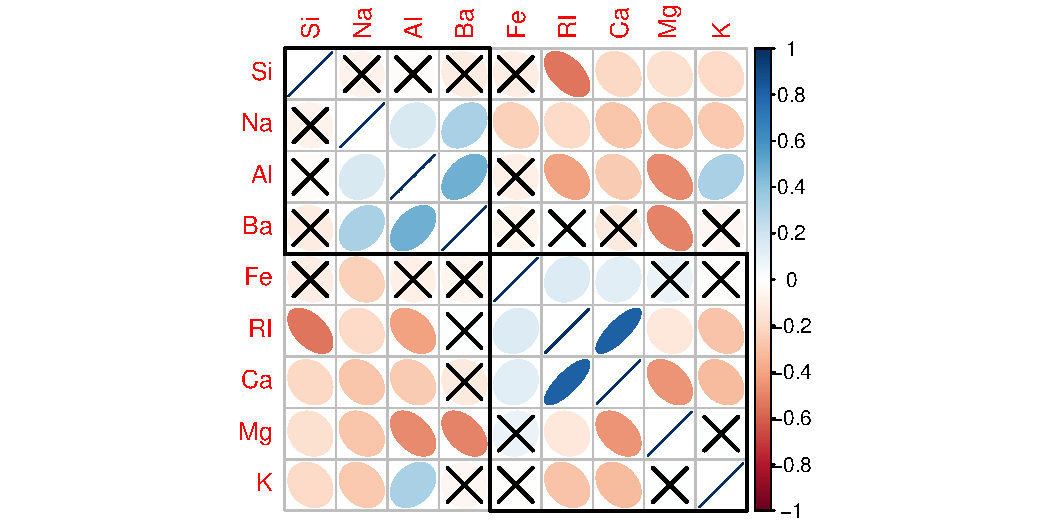
\includegraphics{Carpenter-HW3_files/figure-pdf/unnamed-chunk-16-1.pdf}

}

\end{figure}

\newpage

\begin{enumerate}
\def\labelenumi{\roman{enumi}.}
\setcounter{enumi}{1}
\tightlist
\item
  Provide visualizations of the principal component analysis results
  from the Glass data. Consider incorporating the glass type to group
  and color your biplot.
\end{enumerate}

\begin{Shaded}
\begin{Highlighting}[]
\CommentTok{\# First show the spread of the components}
\FunctionTok{plot}\NormalTok{(pc.glass,}
     \AttributeTok{main =} \StringTok{\textquotesingle{}Principal Components Explanation of Data\textquotesingle{}}\NormalTok{,}
     \AttributeTok{xlab =} \StringTok{\textquotesingle{}Principal Components\textquotesingle{}}\NormalTok{,}
     \AttributeTok{col  =} \StringTok{\textquotesingle{}lightsteelblue3\textquotesingle{}}
\NormalTok{     )}
\end{Highlighting}
\end{Shaded}

\begin{figure}[H]

{\centering 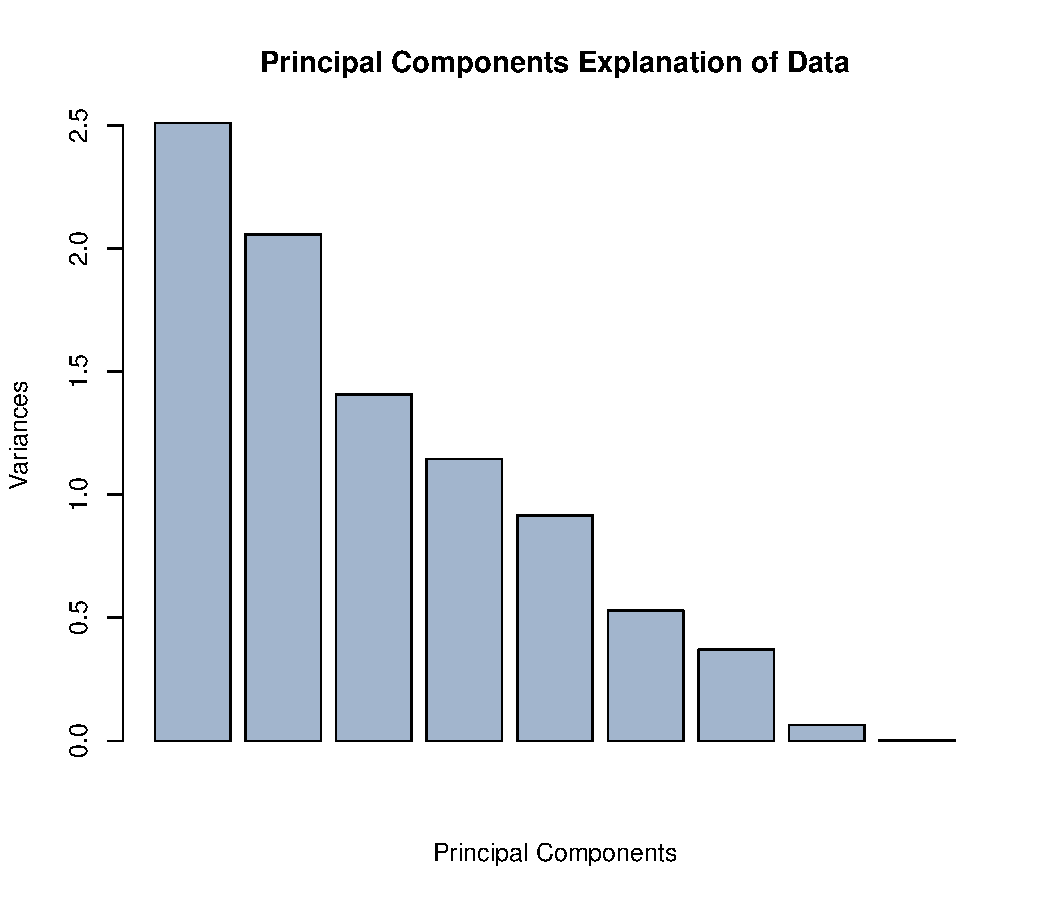
\includegraphics{Carpenter-HW3_files/figure-pdf/unnamed-chunk-18-1.pdf}

}

\end{figure}

\begin{Shaded}
\begin{Highlighting}[]
\CommentTok{\# NExt show the biplots}
\FunctionTok{ggbiplot}\NormalTok{(pc.glass,}
         \AttributeTok{obs.scale    =} \DecValTok{1}\NormalTok{, }
         \AttributeTok{var.scale    =} \DecValTok{1}\NormalTok{, }
         \AttributeTok{varname.size =} \DecValTok{4}\NormalTok{, }
         \AttributeTok{labels.size  =} \DecValTok{10}\NormalTok{, }
         \AttributeTok{circle       =} \ConstantTok{TRUE}\NormalTok{,}
         \AttributeTok{group        =}\NormalTok{ Glass}\SpecialCharTok{$}\NormalTok{Type}\CommentTok{\#,}
         \CommentTok{\# ellipse      = TRUE}
\NormalTok{         ) }\SpecialCharTok{+}
  
  \CommentTok{\# Titles and caption}
  \FunctionTok{labs}\NormalTok{(}\AttributeTok{title   =} \StringTok{\textquotesingle{}Representativeness of First Two Principal Components\textquotesingle{}}\NormalTok{,}
       \AttributeTok{caption =} \StringTok{\textquotesingle{}}\SpecialCharTok{\textbackslash{}n}\StringTok{Using Glass data from mlbench\textquotesingle{}}\NormalTok{) }\SpecialCharTok{+}
  
  \CommentTok{\# Add color to points by glass type}
  \FunctionTok{geom\_point}\NormalTok{(}\FunctionTok{aes}\NormalTok{(}\AttributeTok{colour=}\NormalTok{Glass}\SpecialCharTok{$}\NormalTok{Type), }\AttributeTok{size =} \DecValTok{1}\NormalTok{) }\SpecialCharTok{+}
  
  \CommentTok{\# Categorical palette on glass type}
  \FunctionTok{scale\_color\_brewer}\NormalTok{(}\AttributeTok{name =} \StringTok{\textquotesingle{}Glass Type\textquotesingle{}}\NormalTok{, }
                     \AttributeTok{palette =} \StringTok{\textquotesingle{}Set2\textquotesingle{}}\NormalTok{, }\AttributeTok{type =} \StringTok{\textquotesingle{}qual\textquotesingle{}}\NormalTok{) }\SpecialCharTok{+} 
  
  \FunctionTok{theme\_minimal}\NormalTok{() }\CommentTok{\# the theme}
\end{Highlighting}
\end{Shaded}

\begin{figure}[H]

{\centering 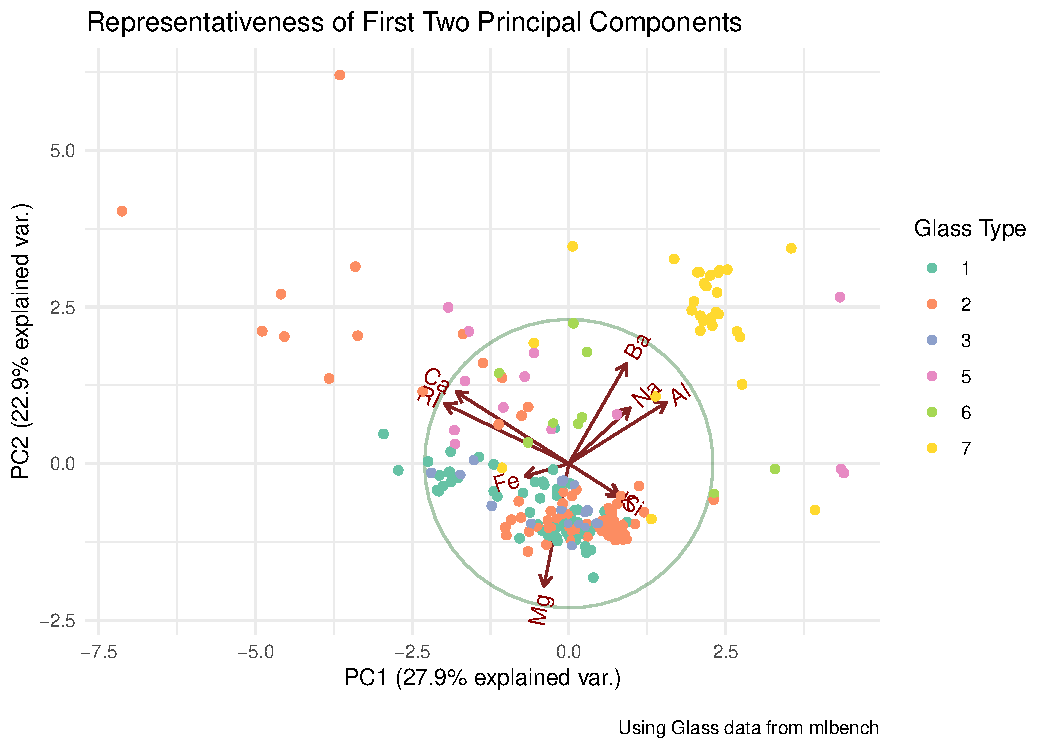
\includegraphics{Carpenter-HW3_files/figure-pdf/unnamed-chunk-20-1.pdf}

}

\end{figure}

\begin{enumerate}
\def\labelenumi{\roman{enumi}.}
\setcounter{enumi}{2}
\tightlist
\item
  Provide an interpretation of the first two prinicpal components the
  Glass data.
\end{enumerate}

\begin{itemize}
\item
  Both PC1 and PC2 represent roughly half (50\%) of the cumulative
  proportion of variance (see summary below)
\item
  PC1 best explains \texttt{Fe}, \texttt{K}, and \texttt{Si} glass
  types, since they lie closest to parallel with the x axis
\item
  PC2 best represents \texttt{Ba}, and \texttt{Mg}, since they lie close
  to parallel with the y axis.
\item
  Other variables appear to be explained by both principal components,
  since they are near a 45 degree angle.
\end{itemize}

Summary of cumulative proportion located here

\begin{Shaded}
\begin{Highlighting}[]
\FunctionTok{summary}\NormalTok{(pc.glass)}
\end{Highlighting}
\end{Shaded}

\begin{verbatim}
Importance of components:
                          PC1    PC2    PC3    PC4    PC5     PC6     PC7
Standard deviation     1.5843 1.4346 1.1864 1.0699 0.9564 0.72704 0.60849
Proportion of Variance 0.2789 0.2287 0.1564 0.1272 0.1016 0.05873 0.04114
Cumulative Proportion  0.2789 0.5076 0.6640 0.7912 0.8928 0.95154 0.99268
                           PC8     PC9
Standard deviation     0.25351 0.04011
Proportion of Variance 0.00714 0.00018
Cumulative Proportion  0.99982 1.00000
\end{verbatim}

\begin{enumerate}
\def\labelenumi{\roman{enumi}.}
\setcounter{enumi}{3}
\tightlist
\item
  Based on the PCA results, do you believe that you can effectively
  reduce the dimension of the data? If so, to what degree? If not, why?
\end{enumerate}

\begin{itemize}
\item
  Given the cumulative proportions above, it is clear that the first two
  principal components capture only half (\textasciitilde50\%) of the
  variation in the original data. We could compare that to a coin flip,
  or a random chance.
\item
  However, the \emph{first four} PC's capture roughly 80\%. This cuts
  the number of variables in half, which is impressive.
\item
  Note that if your \texttt{q} threshold was set to 95\%, then this
  analysis would not perform well, since all but one of the PC's capture
  95\% of the variation in the actual data.
\end{itemize}

\newpage

\hypertarget{c-application-of-lda}{%
\subsection{(c) Application of LDA}\label{c-application-of-lda}}

\begin{enumerate}
\def\labelenumi{\roman{enumi}.}
\item
  Since the Glass data is grouped into various labeled glass types we
  can consider linear discriminant analysis (LDA) as another form of
  dimension reduction. Use the lda method from the MASS package to
  reduce the Glass data dimensionality.
\item
  How would you interpret the first discriminant function, LD1?
\item
  Use the ldahist function from the MASS package to visualize the
  results for LD1 and LD2. Comment on the results.
\end{enumerate}

\newpage

\hypertarget{principal-components-for-dimension-reduction}{%
\section{2. Principal components for dimension
reduction}\label{principal-components-for-dimension-reduction}}

\newpage

\hypertarget{housing-data-dimension-reduction-and-exploration}{%
\section{3. Housing data dimension reduction and
exploration}\label{housing-data-dimension-reduction-and-exploration}}



\end{document}
